\documentclass[a4paper,12pt]{report}

\usepackage{alltt, fancyvrb, url}
\usepackage{graphicx}
\usepackage[utf8]{inputenc}
\usepackage{float}
\usepackage{hyperref}

% Questo commentalo se vuoi scrivere in inglese.
\usepackage[italian]{babel}

\usepackage[italian]{cleveref}

\title{Relazione del progetto di\\Programmazione ad Oggetti\\``Object One Piece''}

\author{De Tommaso Tommaso\\Giorgini Matteo\\Grimaldi Leonardo\\Scorza Edoardo}
\date{\today}


\begin{document}

\maketitle

\begin{abstract}
Questo documento è una relazione di meta livello, ossia una relazione che spiega come scrivere la relazione.
%
Lo scopo di questo documento è quello di aiutare gli studenti a comprendere quali punti trattare nella loro relazione, ed in che modo farlo, evitando di perdere del tempo prezioso in prolisse discussioni di aspetti marginali tralasciando invece aspetti di maggior rilievo.
%
Per ciascuna delle sezioni del documento sarà fornita una descrizione di ciò che ci si aspetta venga prodotto dal team di sviluppo, assieme ad un elenco (per forza di cose non esaustivo) di elementi che \emph{non} dovrebbero essere inclusi.

Il modello della relazione segue il processo tradizionale di ingegneria del software fase per fase (in maniera semplificata).
%
La struttura della relazione non è indicativa ma \textit{obbligatoria}.
%
Gli studenti dovranno produrre un documento che abbia la medesima struttura, non saranno accettati progetti la cui relazione non risponda al requisito suddetto.
%
Lo studente attento dovrebbe sforzarsi di seguire le tappe suggerite in questa relazione anche per l'effettivo sviluppo del progetto: oltre ad una considerevole semplificazione del processo di redazione di questo documento, infatti, il gruppo beneficerà di un processo di sviluppo più solido e collaudato, di tipo top-down.

La meta-relazione verrà fornita corredata di un template \LaTeX{} per coloro che volessero cimentarsi nell'uso.
%
L'uso di \LaTeX{} è vantaggioso per chi ama l'approccio ``what you mean is what you get'', ossia voglia disaccoppiare il contenuto dall'effettivo rendering del documento, accollando al motore \LaTeX{} l'onere di produrre un documento gradevole con la struttura ed il contenuto forniti.
%
Chi non volesse installare l'ambiente di compilazione in locale può valutare l'utilizzo dell'applicazione web \href{https://www.overleaf.com/}{Overleaf}.
%
L'eventuale utilizzo di \LaTeX{} non è fra i requisiti,
non è parte del corso di Programmazione ad Oggetti, e non sarà ovviamente valutato.
%
I docenti accetteranno qualunque relazione in formato standard Portable Document Format (pdf) o Markdown (md), indipendentemente dal software con cui tale documento sarà redatto.

Per la realizzazione degli schemi UML, si raccomanda l'utilizzo di MermaidJS\footnote{\url{https://mermaid.live/}} o PlantUML \footnote{\url{https://plantuml.com/}}.
%
Gli schemi in questa relazione furono realizzati con StarUML.
%
Come per la prosa, non è importante quale strumento sia utilizzato, ma è vitale che gli schemi siano di buona qualità e ben leggibili.

\end{abstract}

\tableofcontents

\chapter{Analisi}

In questo capitolo andrà fatta l'analisi dei requisiti e quella del problema, ossia verranno elencate le cose che l'applicazione dovrà fare (requisiti) e verrà descritto il dominio applicativo (analisi del problema).
%
In fase di analisi, è molto importante tenere a mente che non vi deve essere alcun riferimento al design né tantomeno alle tecnologie implementative, ovvero, non si deve indicare come il software sarà internamente realizzato.
%
La fase di analisi, infatti, \textit{precede} qualunque azione di design o di implementazione.

\section{Requisiti}

Nell'analisi dei \emph{requisiti} dell'applicazione si dovrà spiegare cosa l'applicazione dovrà fare.
%
Non ci si deve concentrare sui particolari problemi, ma esclusivamente su cosa si desidera che l'applicazione faccia.
%
Al termine della lettura della sezione,
il docente deve avere un'idea molto chiara di cosa l'applicazione sia.
%
È consigliato descrivere separatamente i requisiti funzionali (quelli che descrivono l'effettivo
comportamento dell'applicazione) da quelli non funzionali (requisiti che non riguardano direttamente
aspetti comportamentali, come sicurezza, performance, eccetera).

\subsection*{Elementi positivi}
\begin{itemize}
	\item Si fornisce una descrizione in linguaggio naturale di ciò che il software dovrà fare.
	\item Gli obiettivi sono spiegati con chiarezza, per punti.
	\item Se il software è stato commissionato o è destinato ad un utente o compagnia specifici, il committente viene nominato.
	\item Se vi sono termini il cui significato non è immediatamente intuibile, essi vengono spiegati.
	\item Vengono descritti separatamente requisiti funzionali e non funzionali.
	\item Considerato a un paio di pagine un limite ragionevole alla lunghezza della parte sui requisiti, in quello spazio si deve cercare di chiarire \textit{tutti} gli aspetti dell'applicazione, non lasciando decisioni che impattano la parte ``esterna'' alla discussione del design (che dovrebbe solo occuparsi della parte ``interna'').
\end{itemize}

\subsection*{Elementi negativi}
\begin{itemize}
	\item Si forniscono indicazioni circa le soluzioni che si vogliono adottare.
	\item Si forniscono dettagli di tipo tecnico o implementativo (parlando di classi, linguaggi di programmazione, librerie, eccetera).
\end{itemize}

\subsection*{Esempio}
Il software, commissionato dal gestore del centro di ricerca ``Aperture Laboratories Inc.''\footnote{\url{http://aperturescience.com/}}, mira alla costruzione di una intelligenza artificiale di nome GLaDOS (Genetic Lifeform and Disk Operating System).
%
Per intelligenza artificiale si intende un software in grado di assumere decisioni complesse in maniera semi autonoma sugli argomenti di sua competenza, a partire dai vincoli e dagli obiettivi datigli dall'utente.

\subsubsection{Requisiti funzionali}
\begin{itemize}
	\item La suddetta intelligenza artificiale dovrà occuparsi di coordinare le attività all'interno
delle camere di test di Aperture, guidando l'utente attraverso un certo numero di sfide di
difficoltà crescente. Una camera di test è un ambiente realizzato da Aperture Laboratories Inc. al
fine di mettere alla prova le proprie tecnologie di manipolazione dell'ambiente. All'interno della
camera di test, un soggetto qualificato è incaricato di sfruttare gli strumenti messi a
disposizione da Aperture per risolvere alcuni rompicapi. I rompicapi sono di tipo fisico (ad
esempio, manipolazione di oggetti, pressione di pulsanti, azionamento di leve), e si ritengono
conclusi una volta che il soggetto riesce a trovare l'uscita dalla camera di test.
	\item Il piano preciso ed il numero delle sfide sarà variabile, e GLaDOS dovrà essere in grado di adattarsi dinamicamente e di fornire indicazioni di guida.
	\item La personalità di GLaDOS dovrà essere modificabile.
	\item GLaDOS dovrà essere in grado di comunicare col reparto cucina di Aperture, per ordinare torte da donare agli utenti che completassero l'ultima camera di test con successo.
\end{itemize}

\subsubsection{Requisiti non funzionali}
\begin{itemize}
	\item GLaDOS dovrà essere estremamente efficiente nell'uso delle risorse. Le specifiche tecniche parlano della possibilità di funzionare su dispositivi alimentati da una batteria a patata.
\end{itemize}

\section{Analisi e modello del dominio}

In questa sezione si descrive il modello del \textit{dominio
applicativo}, descrivendo le \textit{entità} in gioco ed i rapporti fra loro.
%
Si possono sollevare eventuali aspetti particolarmente impegnativi, descrivendo perché lo sono, senza inserire idee circa possibili soluzioni, ovvero sull'organizzazione interna del software.
%
Infatti, la fase di analisi va effettuata \textbf{prima} del progetto: né il progetto né il software esistono nel momento in cui si effettua l'analisi.
%
La discussione di aspetti propri del software (ossia, della \textit{soluzione} al problema e non del problema stesso) appartengono alla sfera della progettazione, e vanno discussi successivamente.

È obbligatorio fornire uno schema UML del dominio, che diventerà anche lo scheletro della
parte ``entity'' del modello dell'applicazione, ovvero degli elementi costitutivi del modello (in ottica MVC - Model View Controller): se l'analisi è ben fatta, dovreste ottenere una gerarchia di concetti che rappresentano le entità che compongono il problema da risolvere.
%
Un'analisi ben svolta \textbf{prima} di cimentarsi con lo sviluppo rappresenta un notevole aiuto per
le fasi successive: è sufficiente descrivere a parole il dominio, quindi estrarre i sostantivi
utilizzati, capire il loro ruolo all'interno del problema, le relazioni che intercorrono fra loro, e
reificarli in interfacce.

\subsection*{Elementi positivi}
\begin{itemize}
	\item Viene descritto accuratamente il modello del dominio.
	\item Si modella il dominio in forma di UML, descrivendolo appropriatamente.
\end{itemize}

\subsection*{Elementi negativi}
\begin{itemize}
	\item Manca una descrizione a parole del modello del dominio.
	\item Manca una descrizione UML delle entità del dominio e delle relazioni che intercorrono fra loro.
	\item Vengono elencate soluzioni ai problemi, invece della descrizione degli stessi.
	\item Vengono presentati elementi di design, o peggio, aspetti implementativi.
	\item Viene mostrato uno schema UML che include elementi implementativi o non utili alla descrizione del dominio, ma volti alla soluzione (non devono vedersi, ad esempio, campi o metodi privati, o cose che non siano equivalenti ad interfacce).
\end{itemize}

\subsection*{Esempio}
GLaDOS dovrà essere in grado di accedere ad un'insieme di camere di test.
%
Tale insieme di camere prende il nome di percorso.
%
Ciascuna camera è composta di challenge successivi.
%
GLaDOS è responsabile di associare a ciascun challenge un insieme di consigli (suggestions) destinati all'utente (subject), dipendenti da possibili eventi.
%
GLaDOS dovrà poter comunicare coi locali cucina per approntare le torte.
%
Le torte potranno essere dolci, oppure semplici promesse di dolci che verranno disattese.
%
Gli elementi costitutivi il problema sono sintetizzati in \Cref{img:analysis}.

Data la complessità di elaborare consigli via AI senza intervento umano, la prima versione del software fornita prevederà una serie di consigli forniti dall'utente.
%
Il requisito non funzionale riguardante il consumo energetico richiederà studi specifici sulle performance di GLaDOS che non potranno essere effettuati all'interno del monte ore previsto: tale feature sarà oggetto di futuri lavori.

\begin{figure}[H]
\centering{}
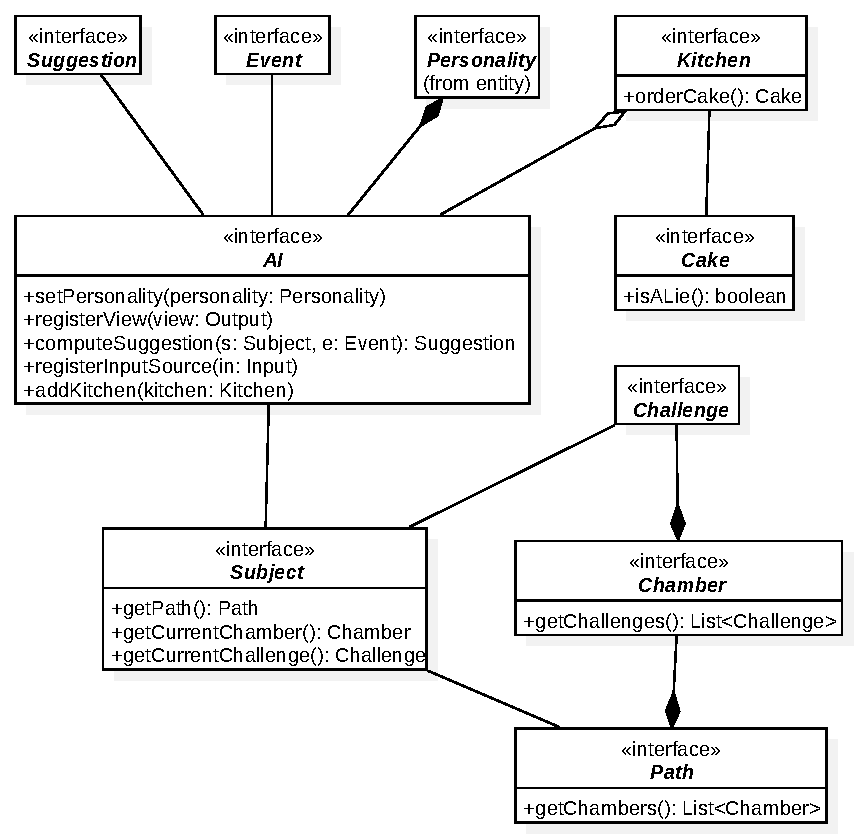
\includegraphics{img/analysis.pdf}
\caption{Schema UML dell'analisi del problema, con rappresentate le entità principali ed i rapporti fra loro}
\label{img:analysis}
\end{figure}

\chapter{Design}

In questo capitolo si spiegano le strategie messe in campo per soddisfare i requisiti identificati nell'analisi.

Si parte da una visione architetturale, il cui scopo è informare il lettore di quale sia il funzionamento dell'applicativo realizzato ad alto livello.
%
In particolare, è necessario descrivere accuratamente in che modo i componenti principali del sistema si coordinano fra loro.
%
A seguire, si dettagliano alcune parti del design, quelle maggiormente rilevanti al fine di chiarificare la logica con cui sono stati affrontati i principali aspetti dell'applicazione.

\section{Architettura}

Questa sezione spiega come le componenti principali del software interagiscono fra loro.
%
In particolare, qui va spiegato \textbf{se} e \textbf{come} è stato utilizzato il pattern
architetturale model-view-controller (e/o alcune sue declinazioni specifiche, come entity-control-boundary).

Se non è stato utilizzato MVC, va spiegata in maniera molto accurata l'architettura scelta, giustificandola in modo appropriato.

Se è stato scelto MVC, vanno identificate con precisione le interfacce e classi che rappresentano i punti d'ingresso per modello, view, e controller.
Raccomandiamo di sfruttare la definizione del dominio fatta in fase di analisi per capire quale sia l'entry point del model, e di non realizzare un'unica macro-interfaccia che, spesso, finisce con l'essere il prodromo ad una ``God class''.
%
Consigliamo anche di separare bene controller e model, facendo attenzione a non includere nel secondo strategie d'uso che appartengono al primo.

In questa sezione vanno descritte, per ciascun componente architetturale che ruoli ricopre (due o tre ruoli al massimo), ed in che modo interagisce (ossia, scambia informazioni) con gli altri componenti dell'architettura.
%
Raccomandiamo di porre particolare attenzione al design dell'interazione fra view e controller: se ben progettato, sostituire in blocco la view non dovrebbe causare alcuna modifica nel controller (tantomeno nel model).

\subsection*{Elementi positivi}
\begin{itemize}
 \item Si mostrano pochi, mirati schemi UML dai quali si deduce con chiarezza quali sono le parti principali del software e come interagiscono fra loro.
 \item Si mette in evidenza se e come il pattern architetturale model-view-controller è stato applicato, anche con l'uso di un UML che mostri le interfacce principali ed i rapporti fra loro.
 \item Si discute se sia semplice o meno, con l'architettura scelta, sostituire in blocco la view: in un MVC ben fatto, controller e modello non dovrebbero in alcun modo cambiare se si transitasse da una libreria grafica ad un'altra (ad esempio, da Swing a JavaFX, o viceversa).
\end{itemize}

\subsection*{Elementi negativi}
\begin{itemize}
 \item L'architettura è fatta in modo che sia impossibile riusare il modello per un software diverso che affronta lo stesso problema.
 \item L'architettura è tale che l'aggiunta di una funzionalità sul controller impatta pesantemente su view e/o modello.
 \item L'architettura è tale che la sostituzione in blocco della view impatta sul controller o, peggio ancora, sul modello.
 \item Si presentano UML caotici, difficili da leggere.
 \item Si presentano UML in cui sono mostrati elementi di dettaglio non appartenenti all'architettura, ad esempio includenti campi o con metodi che non interessano la parte di interazione fra le componenti principali del software.
 \item Si presentano schemi UML con classi (nel senso UML del termine) che ``galleggiano'' nello schema, non connesse, ossia senza relazioni con il resto degli elementi inseriti.
 \item Si presentano elementi di design di dettaglio, ad esempio tutte le classi e interfacce del modello o della view.
 \item Si discutono aspetti implementativi, ad esempio eventuali librerie usate oppure dettagli di codice.
\end{itemize}

\subsection*{Esempio}

L'architettura di GLaDOS segue il pattern architetturale MVC.
%
Più nello specifico, a livello architetturale, si è scelto di utilizzare MVC in forma ``ECB'', ossia ``entity-control-boundary''\footnote{
Si fa presente che il pattern ECB effettivamente esiste in letteratura come ``istanza'' di MVC, e chi volesse può utilizzarlo come reificazione di MVC.
}.
%
GLaDOS implementa l'interfaccia AI, ed è il controller del sistema.
Essendo una intelligenza artificiale, è una classe attiva.
%
GLaDOS accetta la registrazione di Input ed Output, che fanno parte della ``view'' di MVC, e sono il ``boundary'' di ECB.
Gli Input rappresentano delle nuove informazioni che vengono fornite all'IA, ad esempio delle modifiche nel valore di un sensore, oppure un comando da parte dell'operatore.
Questi input infatti forniscono eventi.
Ottenere un evento è un'operazione bloccante: chi la esegue resta in attesa di un effettivo evento.
Di fatto, quindi, GLaDOS si configura come entità \textit{reattiva}.
Ogni volta che c'è un cambio alla situazione del soggetto, GLaDOS notifica i suoi Output,
informandoli su quale sia la situazione corrente.
%
Conseguentemente, GLaDOS è un ``observable'' per Output.

\begin{figure}[h]
\centering{}
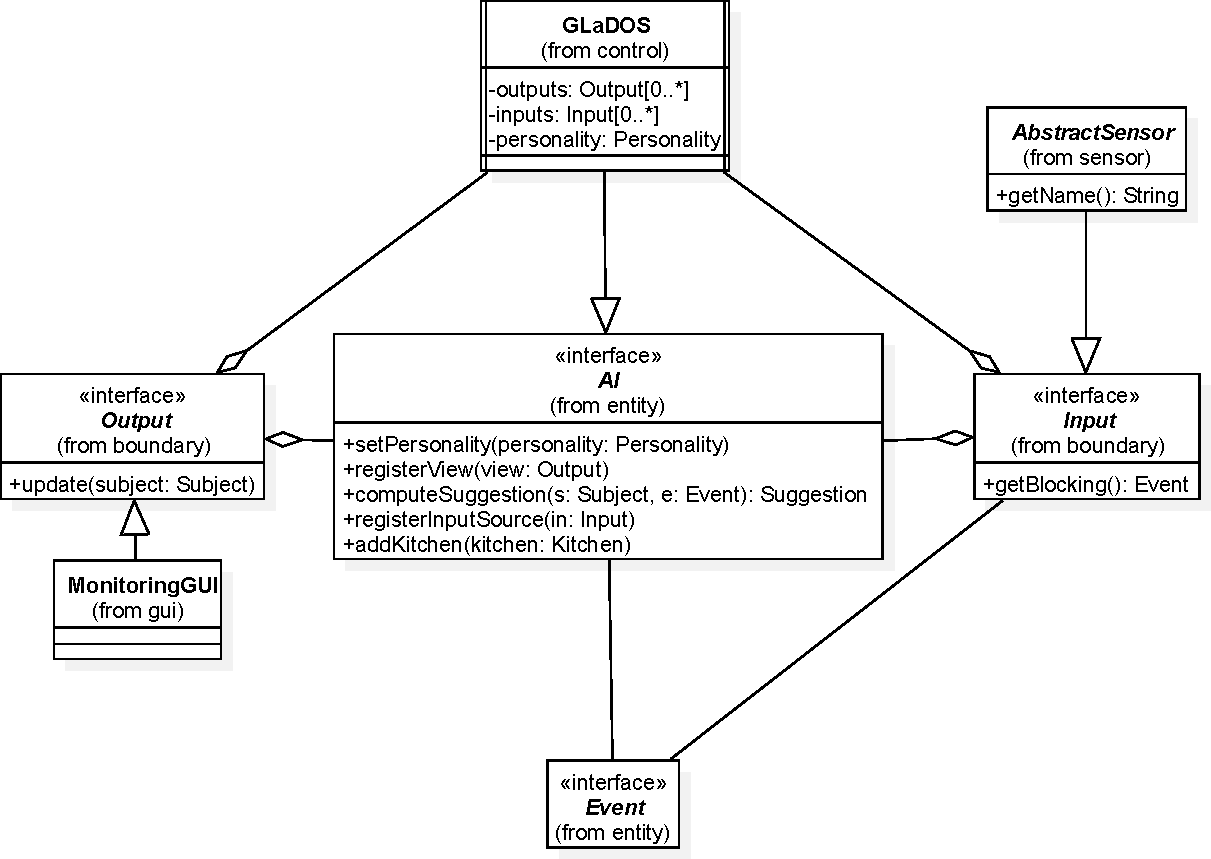
\includegraphics[width=\textwidth]{img/arch}
\caption{Schema UML architetturale di GLaDOS. L'interfaccia \texttt{GLaDOS} è il controller del sistema, mentre \texttt{Input} ed \texttt{Output} sono le interfacce che mappano la view (o, più correttamente in questo specifico esempio, il boundary). Un'eventuale interfaccia grafica interattiva dovrà implementarle entrambe.}
\label{img:goodarch}
\end{figure}

Con questa architettura, possono essere aggiunti un numero arbitrario di input ed output
all'intelligenza artificiale.
%
Ovviamente, mentre l'aggiunta di output è semplice e non richiede alcuna modifica all'IA, la
presenza di nuovi tipi di evento richiede invece in potenza aggiunte o rifiniture a GLaDOS.
%
Questo è dovuto al fatto che nuovi Input rappresentano di fatto nuovi elementi della business
logic, la cui alterazione od espansione inevitabilmente impatta il controller del progetto.

In \Cref{img:goodarch} è esemplificato il diagramma UML architetturale.


\section{Design dettagliato}

In questa sezione si possono approfondire alcuni elementi del design con maggior dettaglio.
%
Mentre ci attendiamo principalmente (o solo) interfacce negli schemi UML delle sezioni precedenti,
in questa sezione è necessario scendere in maggior dettaglio presentando la struttura di alcune sottoparti rilevanti dell'applicazione.
%
È molto importante che, descrivendo la soluzione ad un problema, quando possibile si mostri che non si è re-inventata la ruota ma si è applicato un design pattern noto.
%
Che si sia utilizzato (o riconosciuto) o meno un pattern noto, è comunque bene definire qual è il problema che si è affrontato, qual è la soluzione messa in campo, e quali motivazioni l'hanno spinta.
%
È assolutamente inutile, ed è anzi controproducente, descrivere classe-per-classe (o peggio ancora metodo-per-metodo) com'è fatto il vostro software: è un livello di dettaglio proprio della documentazione dell'API (deducibile dalla Javadoc).

\textbf{È necessario che ciascun membro del gruppo abbia una propria sezione di design dettagliato,
di cui sarà il solo responsabile}.
%
Ciascun autore dovrà spiegare in modo corretto e giustamente approfondito (non troppo in dettaglio, non superficialmente) il proprio contributo.
%
È importante focalizzarsi sulle scelte che hanno un impatto positivo sul riuso, sull'estensibilità, e sulla chiarezza dell'applicazione.
%
Esattamente come nessun ingegnere meccanico presenta un solo foglio con l'intero progetto di una vettura di Formula 1, ma molteplici fogli di progetto che mostrano a livelli di dettaglio differenti le varie parti della vettura e le modalità di connessione fra le parti, così ci aspettiamo che voi, futuri ingegneri informatici, ci presentiate prima una visione globale del progetto, e via via siate in grado di dettagliare le singole parti, scartando i componenti che non interessano quella in esame.
%
Per continuare il parallelo con la vettura di Formula 1, se nei fogli di progetto che mostrano il
design delle sospensioni anteriori appaiono pezzi che appartengono al volante o al turbo, c'è una
chiara indicazione di qualche problema di design.

Si divida la sezione in sottosezioni, e per ogni aspetto di design che si vuole approfondire, si presenti:
\begin{enumerate}
    \item: una breve descrizione in linguaggio naturale del problema che si vuole risolvere, se necessario ci si può aiutare con schemi o immagini;
    \item: una descrizione della soluzione proposta, analizzando eventuali alternative che sono state prese in considerazione, e che descriva pro e contro della scelta fatta;
    \item: uno schema UML che aiuti a comprendere la soluzione sopra descritta;
    \item: se la soluzione è stata realizzata utilizzando uno o più pattern noti, si spieghi come questi sono reificati nel progetto
    (ad esempio: nel caso di Template Method, qual è il metodo template;
    nel caso di Strategy, quale interfaccia del progetto rappresenta la strategia, e quali sono le sue implementazioni;
    nel caso di Decorator, qual è la classe astratta che fa da Decorator e quali sono le sue implementazioni concrete; eccetera);
\end{enumerate}
%
La presenza di pattern di progettazione \emph{correttamente utilizzati} è valutata molto positivamente.
%
L'uso inappropriato è invece valutato negativamente: a tal proposito, si raccomanda di porre particolare attenzione all'abuso di Singleton, che, se usato in modo inappropriato, è di fatto un anti-pattern.

\subsection*{Elementi positivi}

\begin{itemize}
	\item Ogni membro del gruppo discute le proprie decisioni di progettazione, ed in particolare le azioni volte ad anticipare possibili cambiamenti futuri (ad esempio l'aggiunta di una nuova funzionalità, o il miglioramento di una esistente).
	\item Si mostrano le principali interazioni fra le varie componenti che collaborano alla soluzione di un determinato problema.
	\item Si identificano, utilizzano \textit{appropriatamente}, e descrivono diversi design pattern.
	\item Ogni membro del gruppo identifica i pattern utilizzati nella sua sottoparte.
	\item Si mostrano gli aspetti di design più rilevanti dell'applicazione, mettendo in luce la maniera in cui si è costruita la soluzione ai problemi descritti nell'analisi.
	\item Si tralasciano aspetti strettamente implementativi e quelli non rilevanti, non mostrandoli negli schemi UML (ad esempio, campi privati) e non descrivendoli.
	\item Ciascun elemento di design identificato presenta una piccola descrizione del problema calato
nell'applicazione, uno schema UML che ne mostra la concretizzazione nelle classi del progetto, ed
una breve descrizione della motivazione per cui tale soluzione è stata scelta, specialmente se è stato utilizzato un pattern noto. Ad esempio, se si
dichiara di aver usato Observer, è necessario specificare chi sia l'observable e chi l'observer; se
si usa Template Method, è necessario indicare quale sia il metodo template; se si usa Strategy, è
necessario identificare l'interfaccia che rappresenta la strategia; e via dicendo.
\end{itemize}

\subsection*{Elementi negativi}
\begin{itemize}
	\item Il design del modello risulta scorrelato dal problema descritto in analisi.
	\item Si tratta in modo prolisso, classe per classe, il software realizzato, o comunque si riduce la sezione ad un mero elenco di quanto fatto.
	\item Non si presentano schemi UML esemplificativi.
	\item Non si individuano design pattern, o si individuano in modo errato (si spaccia per design pattern qualcosa che non lo è).
	\item Si utilizzano design pattern in modo inopportuno. Un esempio classico è l'abuso di
Singleton per entità che possono essere univoche ma non devono necessariamente esserlo. Si rammenta
che Singleton ha senso nel secondo caso (ad esempio \texttt{System} e \texttt{Runtime} sono
singleton), mentre rischia di essere un problema nel secondo. Ad esempio, se si rendesse singleton
il motore di un videogioco, sarebbe impossibile riusarlo per costruire un server per partite online
(dove, presumibilmente, si gestiscono parallelamente più partite).
	\item Si producono schemi UML caotici e difficili da leggere, che comprendono inutili elementi di dettaglio.
	\item Si presentano schemi UML con classi (nel senso UML del termine) che ``galleggiano'' nello schema, non connesse, ossia senza relazioni con il resto degli elementi inseriti.
	\item Si tratta in modo inutilmente prolisso la divisione in package, elencando ad esempio le classi una per una.
\end{itemize}

\subsection*{Esempio minimale (e quindi parziale) di sezione di progetto con UML ben realizzati}

\subsubsection{Personalità intercambiabili}

\begin{figure}[H]
\centering{}
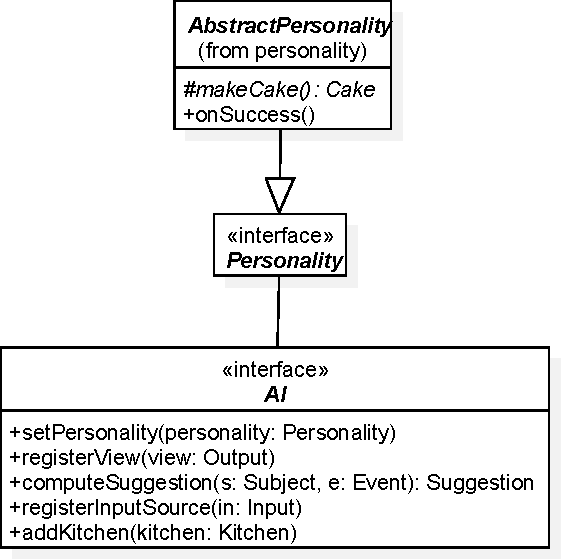
\includegraphics[width=\textwidth]{img/strategy}
\caption{Rappresentazione UML del pattern Strategy per la personalità di GLaDOS}
\label{img:strategy}
\end{figure}

\paragraph{Problema} GLaDOS ha più personalità intercambiabili, la cui presenza deve essere trasparente al client.

\paragraph{Soluzione} Il sistema per la gestione della personalità utilizza il \textit{pattern Strategy}, come da
\Cref{img:strategy}: le implementazioni di \texttt{Personality} possono essere modificate, e la
modifica impatta direttamente sul comportamento di GLaDOS.

\subsubsection{Riuso del codice delle personalità}

\begin{figure}[H]
\centering{}
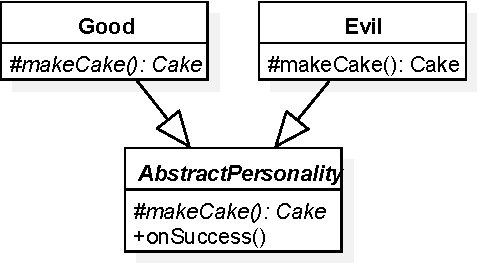
\includegraphics[width=\textwidth]{img/template}
\caption{Rappresentazione UML dell'applicazione del pattern Template Method alla gerarchia delle Personalità}
\label{img:template}
\end{figure}

\paragraph{Problema} In fase di sviluppo, sono state sviluppate due personalità, una buona ed una cattiva.
Quella buona restituisce sempre una torta vera, mentre quella cattiva restituisce sempre la
promessa di una torta che verrà in realtà disattesa.
Ci si è accorti che diverse personalità condividevano molto del comportamento,
portando a classi molto simili e a duplicazione.

\paragraph{Soluzione} Dato che le due personalità differiscono solo per il comportamento da effettuarsi in caso di percorso completato con successo,
è stato utilizzato il \textit{pattern template method} per massimizzare il riuso, come da \Cref{img:template}.
Il metodo template è \texttt{onSuccess()}, che chiama un metodo astratto e protetto
\texttt{makeCake()}.

\subsubsection{Gestione di output multipli}

\begin{figure}[H]
\centering{}
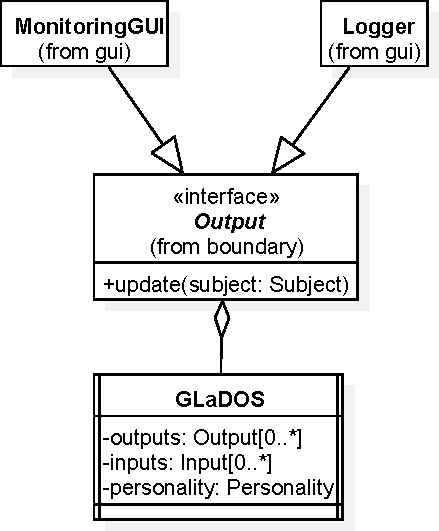
\includegraphics[width=.7\textwidth]{img/observer}
\caption{Il pattern Observer è usato per consentire a GLaDOS di informare tutti i sistemi di output in ascolto}
\label{img:observer}
\end{figure}

\paragraph{Problema} Il sistema deve supportare output multipli. In particolare, si richiede che vi sia un logger che stampa a terminale o su file,
e un'interfaccia grafica che mostri una rappresentazione grafica del sistema.

\paragraph{Soluzione} Dato che i due sistemi di reporting utilizzano le medesime informazioni, si è deciso di raggrupparli dietro l'interfaccia \texttt{Output}.
A questo punto, le due possibilità erano quelle di far sì che \texttt{GLaDOS} potesse pilotarle entrambe.
Invece di fare un sistema in cui questi output sono obbligatori e connessi, si è deciso di usare maggior flessibilità (anche in vista di future estensioni)
e di adottare una comunicazione uno-a-molti fra \texttt{GLaDOS} ed i sistemi di output.
La scelta è quindi ricaduta sul \textit{pattern Observer}: \texttt{GLaDOS} è observable, e le istanze di \texttt{Output} sono observer.
%
Il suo utilizzo è esemplificato in \Cref{img:observer}


\subsection*{Contro-esempio: pessimo diagramma UML}

In \Cref{img:badarch} è mostrato il modo \textbf{sbagliato} di fare le cose.
%
Questo schema è fatto male perché:
\begin{itemize}
	\item È caotico.
	\item È difficile da leggere e capire.
	\item Vi sono troppe classi, e non si capisce bene quali siano i rapporti che intercorrono fra loro.
	\item Si mostrano elementi implementativi irrilevanti, come i campi e i metodi privati nella classe \texttt{AbstractEnvironment}.
	\item Se l'intenzione era quella di costruire un diagramma architetturale, allora lo schema è ancora più sbagliato, perché mostra pezzi di implementazione.
	\item Una delle classi, in alto al centro, galleggia nello schema, non connessa a nessuna altra classe, e di fatto costituisce da sola un secondo schema UML scorrelato al resto
	\item Le interfacce presentano tutti i metodi e non una selezione che aiuti il lettore a capire quale parte del sistema si vuol mostrare.
\end{itemize}


\begin{figure}[h]
\centering{}
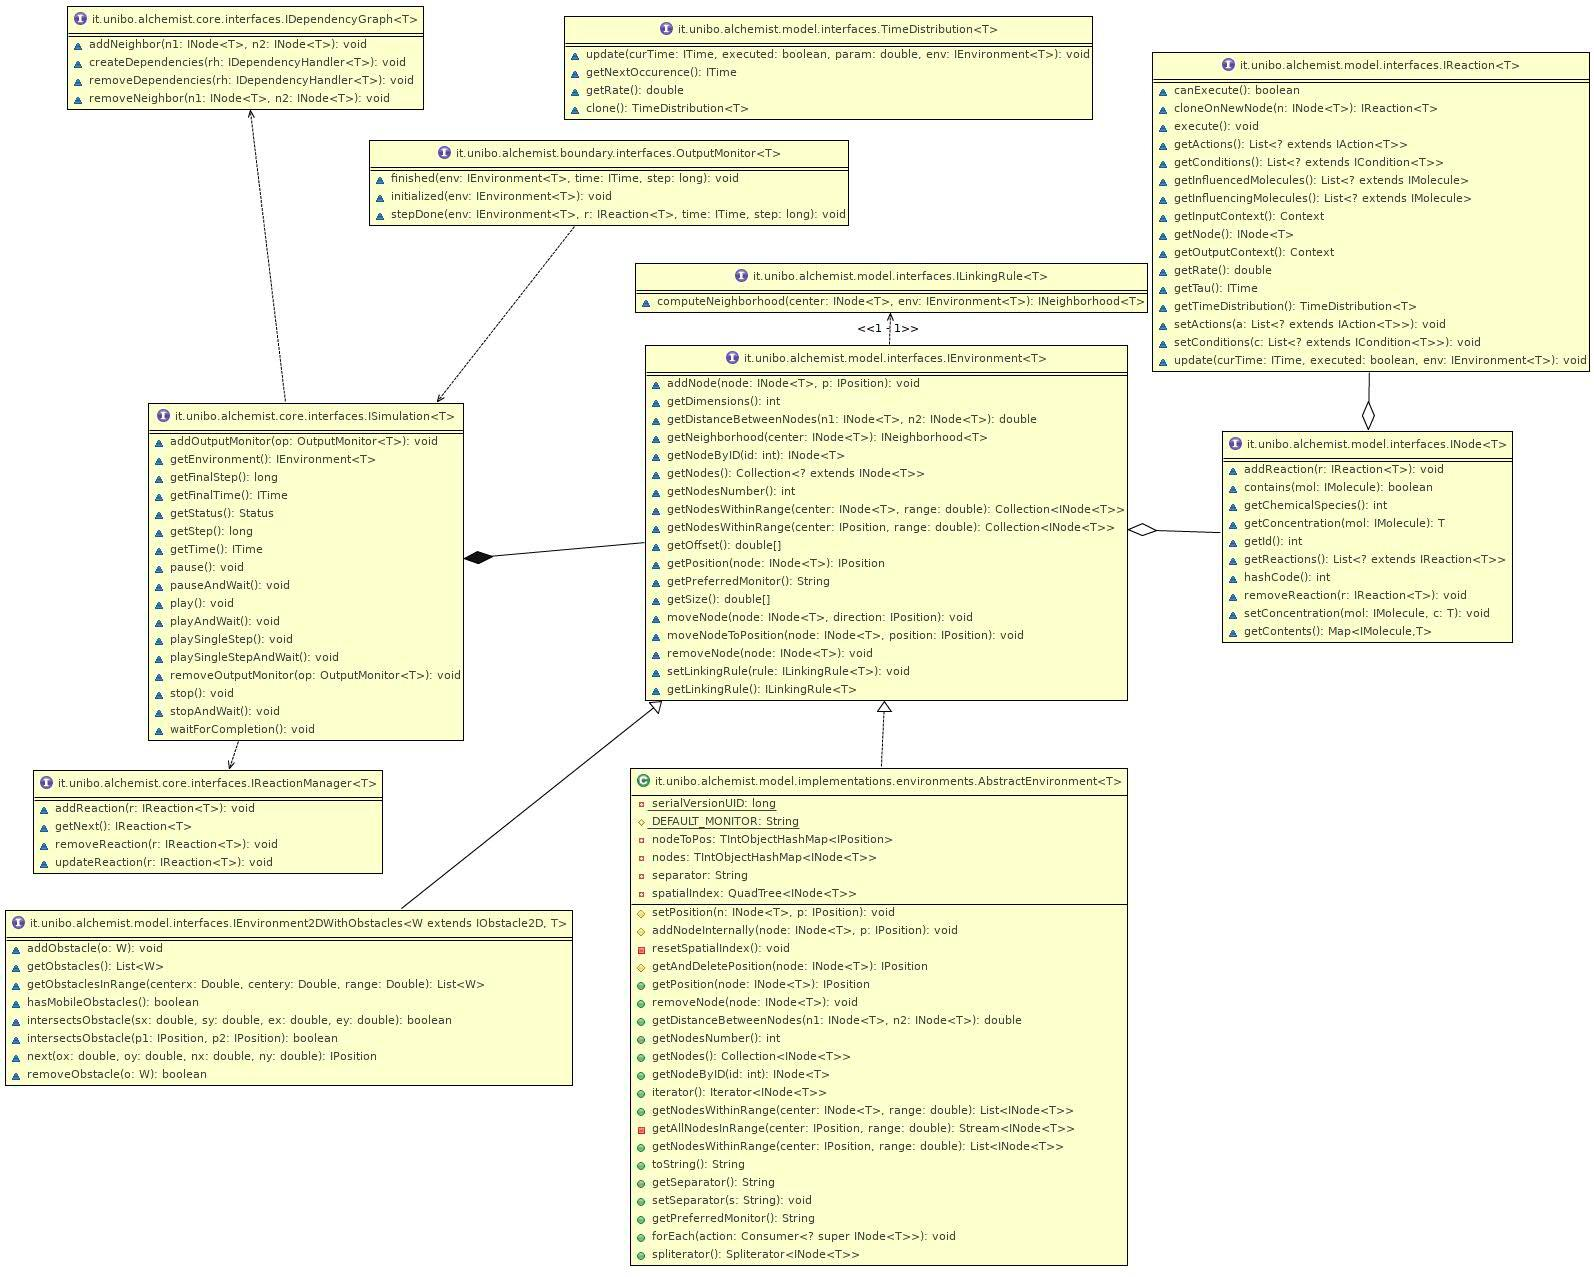
\includegraphics[width=\textwidth]{img/badarch}
\caption{Schema UML mal fatto e con una pessima descrizione, che non aiuta a capire. Don't try this at home.}
\label{img:badarch}
\end{figure}


\chapter{Sviluppo}
\section{Testing automatizzato}

Il testing automatizzato è un requisito di qualunque progetto software che si rispetti, e consente di verificare che non vi siano regressioni nelle funzionalità a fronte di aggiornamenti.
%
Per quanto riguarda questo progetto è considerato sufficiente un test minimale, a patto che sia completamente automatico.
%
Test che richiedono l'intervento da parte dell'utente sono considerati \textit{negativamente} nel computo del punteggio finale.

\subsection*{Elementi positivi}

\begin{itemize}
 \item Si descrivono molto brevemente i componenti che si è deciso di sottoporre a test automatizzato.
 \item Si utilizzano suite specifiche (e.g. JUnit) per il testing automatico.
\end{itemize}

\subsection*{Elementi negativi}
\begin{itemize}
 \item Non si realizza alcun test automatico.
 \item La non presenza di testing viene aggravata dall'adduzione di motivazioni non valide. Ad esempio, si scrive che l'interfaccia grafica non è testata automaticamente perché è \emph{impossibile} farlo\footnote{Testare in modo automatico le interfacce grafiche è possibile (si veda, come esempio, \url{https://github.com/TestFX/TestFX}), semplicemente nel corso non c'è modo e tempo di introdurvi questo livello di complessità. Il fatto che non vi sia stato insegnato come farlo non implica che sia impossibile!}.
 \item Si descrive un testing di tipo manuale in maniera prolissa.
 \item Si descrivono test effettuati manualmente che sarebbero potuti essere automatizzati, ad esempio scrivendo che si è usata l'applicazione manualmente.
 \item Si descrivono test non presenti nei sorgenti del progetto.
 \item I test, quando eseguiti, falliscono.
\end{itemize}

\section{Note di sviluppo}

Questa sezione, come quella riguardante il design dettagliato va svolta \textbf{singolarmente da ogni membro del gruppo}.
%
Nella prima parte, ciascuno dovrà mostrare degli esempi di codice particolarmente ben realizzati,
che dimostrino proefficienza con funzionalità avanzate del linguaggio e capacità di spingersi oltre le librerie mostrate a lezione.

\begin{itemize}
	\item \textbf{Elencare} (fare un semplice elenco per punti, non un testo!) le feature \textit{avanzate} del linguaggio e dell'ecosistema Java che sono state
utilizzate. Le feature di interesse sono:
	\begin{itemize}
		\item Progettazione con generici, ad esempio costruzione di nuovi tipi generici, e uso di generici bounded.
		L'uso di classi generiche di libreria non è considerato avanzato.
		\item Uso di lambda expressions
		\item Uso di \texttt{Stream}, di \texttt{Optional} o di altri costrutti funzionali
		\item Uso di reflection
		\item Definizione ed uso di nuove annotazioni
		\item Uso del Java Platform Module System
		\item Uso di parti della libreria JDK non spiegate a lezione (networking, compressione, parsing XML, eccetera...)
		\item Uso di librerie di terze parti (incluso JavaFX): Google Guava, Apache Commons...
	\end{itemize}
	\item Si faccia molta attenzione a non scrivere banalità, elencando qui features di tipo ``core'', come le eccezioni, le enumerazioni, o le inner class: nessuna di queste è considerata avanzata.
	\item Per ogni feature avanzata, mostrata, includere:
	\begin{itemize}
		\item Nome della feature
		\item Permalink GitHub al punto nel codice in cui è stata utilizzata
	\end{itemize}
\end{itemize}

In questa sezione, \textit{dopo l'elenco},
vanno menzionati ed attributi con precisione eventuali pezzi di codice ``riadattati'' (o scopiazzati...) da Internet o da altri progetti,
pratica che tolleriamo ma che non raccomandiamo.
%
Si rammenta agli studenti che non è consentito partire da progetti esistenti e procedere per modifiche successive.
%
Si ricorda anche che i docenti hanno in mano strumenti antiplagio piuttosto raffinati e che ``capiscono'' il codice e la storia delle modifiche del progetto,
per cui tecniche banali come cambiare nomi (di classi, metodi, campi, parametri, o variabili locali),
aggiungere o togliere commenti,
oppure riordinare i membri di una classe vengono individuate senza problemi.
%
Le regole del progetto spiegano in dettaglio l'approccio dei docenti verso atti gravi come il plagiarismo.

I pattern di design \textbf{non} vanno messi qui.
%
L'uso di pattern di design (come suggerisce il nome) è un aspetto avanzato di design, non di implementazione,
e non va in questa sezione.

\subsection*{Elementi positivi}

\begin{itemize}
	\item Si elencano gli aspetti avanzati di linguaggio che sono stati impiegati
	\item Si elencano le librerie che sono state utilizzate
	\item Per ciascun elemento, si fornisce un permalink
	\item Ogni permalink fa riferimento ad uno snippet di codice scritto dall'autore della sezione (i docenti verificheranno usando \texttt{git blame})
	\item Se si è utilizzato un particolare algoritmo, se ne cita la fonte originale.
	Ad esempio, se si è usato Mersenne Twister per la generazione di numeri pseudo-random, si cita \cite{mersenne}.
	\item Si identificano parti di codice prese da altri progetti, dal web, o comunque scritte in forma originale da altre persone.
	In tal senso, si ricorda che agli ingegneri non è richiesto di re-inventare la ruota continuamente:
	se si cita debitamente la sorgente è tollerato fare uso di di snippet di codice open source per risolvere velocemente problemi non banali.
	Nel caso in cui si usino snippet di codice di qualità discutibile,
	oltre a menzionarne l'autore originale si invitano gli studenti ad adeguare tali parti di codice agli standard e allo stile del progetto.
	Contestualmente, si fa presente che è largamente meglio fare uso di una libreria che copiarsi pezzi di codice:
	qualora vi sia scelta (e tipicamente c'è), si preferisca la prima via.
\end{itemize}

\subsection*{Elementi negativi}
\begin{itemize}
	\item Si elencano feature core del linguaggio invece di quelle segnalate. Esempi di feature core da non menzionare sono:
    \begin{itemize}
        \item eccezioni;
        \item classi innestate;
        \item enumerazioni;
        \item interfacce.
    \end{itemize}
	\item Si elencano applicazioni di terze parti (peggio se per usarle occorre licenza, e lo studente ne è sprovvisto) che non c'entrano nulla con lo sviluppo, ad esempio:
    \begin{itemize}
        \item Editor di grafica vettoriale come Inkscape o Adobe Illustrator;
        \item Editor di grafica scalare come GIMP o Adobe Photoshop;
        \item Editor di audio come Audacity;
        \item Strumenti di design dell'interfaccia grafica come SceneBuilder: il codice è in ogni caso inteso come sviluppato da voi.
    \end{itemize}
	\item Si descrivono aspetti di scarsa rilevanza, o si scende in dettagli inutili.
	\item Sono presenti parti di codice sviluppate originalmente da altri che non vengono debitamente segnalate.
	In tal senso, si ricorda agli studenti che i docenti hanno accesso a tutti i progetti degli anni passati,
	a Stack Overflow,
	ai principali blog di sviluppatori ed esperti Java,
	ai blog dedicati allo sviluppo di soluzioni e applicazioni
	(inclusi blog dedicati ad Android e allo sviluppo di videogame),
	nonché ai vari GitHub, GitLab, e Bitbucket.
	Conseguentemente, è \emph{molto} conveniente \emph{citare} una fonte ed usarla invece di tentare di spacciare per proprio il lavoro di altri.
	\item Si elencano design pattern
\end{itemize}

\subsection{Esempio}

\subsubsection{Utilizzo della libreria SLF4J}

Utilizzata in vari punti.
Un esempio è \url{https://github.com/AlchemistSimulator/Alchemist/blob/5c17f8b76920c78d955d478864ac1f11508ed9ad/alchemist-swingui/src/main/java/it/unibo/alchemist/boundary/swingui/effect/impl/EffectBuilder.java#L49}

\subsubsection{Utilizzo di \texttt{LoadingCache} dalla libreria Google Guava}

Permalink: \url{https://github.com/AlchemistSimulator/Alchemist/blob/d8a1799027d7d685569e15316a32e6394632ce71/alchemist-incarnation-protelis/src/main/java/it/unibo/alchemist/protelis/AlchemistExecutionContext.java#L141-L143}

\subsubsection{Utilizzo di \texttt{Stream} e lambda expressions}

Usate pervasivamente. Il seguente è un singolo esempio.
Permalink: \url{https://github.com/AlchemistSimulator/Alchemist/blob/d8a1799027d7d685569e15316a32e6394632ce71/alchemist-incarnation-protelis/src/main/java/it/unibo/alchemist/model/ProtelisIncarnation.java#L98-L120}

\subsubsection{Scrittura di metodo generico con parametri contravarianti}

Permalink: \url{https://github.com/AlchemistSimulator/Alchemist/blob/d8a1799027d7d685569e15316a32e6394632ce71/alchemist-incarnation-protelis/src/main/java/it/unibo/alchemist/protelis/AlchemistExecutionContext.java#L141-L143}

\subsubsection{Protezione da corse critiche usando \texttt{Semaphore}}

Permalink: \url{https://github.com/AlchemistSimulator/Alchemist/blob/d8a1799027d7d685569e15316a32e6394632ce71/alchemist-incarnation-protelis/src/main/java/it/unibo/alchemist/model/ProtelisIncarnation.java#L388-L440}


\chapter{Commenti finali}

In quest'ultimo capitolo si tirano le somme del lavoro svolto e si delineano eventuali sviluppi
futuri.

\textit{Nessuna delle informazioni incluse in questo capitolo verrà utilizzata per formulare la valutazione finale}, a meno che non sia assente o manchino delle sezioni obbligatorie.
%
Al fine di evitare pregiudizi involontari, l'intero capitolo verrà letto dai docenti solo dopo aver formulato la valutazione.

\section{Autovalutazione e lavori futuri}

\textbf{È richiesta una sezione per ciascun membro del gruppo, obbligatoriamente}.
%
Ciascuno dovrà autovalutare il proprio lavoro, elencando i punti di forza e di debolezza in quanto prodotto.
Si dovrà anche cercare di descrivere \emph{in modo quanto più obiettivo possibile} il proprio ruolo all'interno del gruppo.
Si ricorda, a tal proposito, che ciascuno studente è responsabile solo della propria sezione: non è un problema se ci sono opinioni contrastanti, a patto che rispecchino effettivamente l'opinione di chi le scrive.
Nel caso in cui si pensasse di portare avanti il progetto, ad esempio perché effettivamente impiegato, o perché sufficientemente ben riuscito da poter esser usato come dimostrazione di esser capaci progettisti, si descriva brevemente verso che direzione portarlo.

\section{Difficoltà incontrate e commenti per i docenti}

Questa sezione, \textbf{opzionale}, può essere utilizzata per segnalare ai docenti eventuali problemi o difficoltà incontrate nel corso o nello svolgimento del progetto, può essere vista come una seconda possibilità di valutare il corso (dopo quella offerta dalle rilevazioni della didattica) avendo anche conoscenza delle modalità e delle difficoltà collegate all'esame, cosa impossibile da fare usando le valutazioni in aula per ovvie ragioni.
%
È possibile che alcuni dei commenti forniti vengano utilizzati per migliorare il corso in futuro: sebbene non andrà a vostro beneficio, potreste fare un favore ai vostri futuri colleghi.
%
Ovviamente \textit{il contenuto della sezione non impatterà il voto finale}.

\appendix
\chapter{Guida utente}

Capitolo in cui si spiega come utilizzare il software. Nel caso in cui il suo uso sia del tutto
banale, tale capitolo può essere omesso.
%
A tal riguardo, si fa presente agli studenti che i docenti non hanno mai utilizzato il software
prima, per cui aspetti che sembrano del tutto banali a chi ha sviluppato l'applicazione possono non
esserlo per chi la usa per la prima volta.
%
Se, ad esempio, per cominciare una partita con un videogioco è necessario premere la barra
spaziatrice, o il tasto ``P'', è necessario che gli studenti lo segnalino.

%%
Avviando il gioco, l'utente si troverà sullo schermo una finestra con in centro una griglia blu (mappa di gioco) e un HUD sulla parte destra.
%
La griglia
\subsection*{Elementi positivi}

\begin{itemize}
 \item Si istruisce in modo semplice l'utente sull'uso dell'applicazione, eventualmente facendo uso di schermate e descrizioni.
\end{itemize}

\subsection*{Elementi negativi}
\begin{itemize}
 \item Si descrivono in modo eccessivamente minuzioso tutte le caratteristiche, anche minori, del software in oggetto.
 \item Manca una descrizione che consenta ad un utente qualunque di utilizzare almeno le funzionalità primarie dell'applicativo.
\end{itemize}

\chapter{Esercitazioni di laboratorio}

In questo capitolo ciascuno studente elenca gli esercizi di laboratorio che ha svolto
(se ne ha svolti),
elencando i permalink dei post sul forum dove è avvenuta la consegna.
%
Questa sezione potrebbe essere processata da strumenti automatici,
per cui link a oggetti diversi dal permalink della consegna,
errori nell'email o nel nome del laboratorio possono portare ad ignorare alcune consegne,
si raccomanda la massima precisione.

\subsection{leonardo.grimaldi2@studio.unibo.it}

\begin{itemize}
 \item Laboratorio 08: \url{https://virtuale.unibo.it/mod/forum/discuss.php?d=148025#p209751}
\end{itemize}

\bibliographystyle{alpha}
\bibliography{13-template}

\end{document}
